\documentclass[a4paper,notitlepage]{article}
\usepackage{ssn-format}
\title{PFS ICS network connections}
\author{PFS ICS}
\date{2014--08--06}
\begin{document}

%\drafttrue
\SSNID{00002}
\SSNREV{002}
\SSNCATEGORY{ICS}
\SSNChangeRecord{
    Rev.2  / TUE-Opt stand-by, IR4(SpS) / 2014--08--06 \\ 
    Rev.1b / First Release (DRAFT rev.b) / 2014--01--22}
\SSNReference{(none)}
\SSNAttachment{(none)}
\SSNWritten{Atsushi Shimono}

\ssnhead

\section{Abstract}

This is not an organized ICD, but is written to have mutual understanding 
what network connection we need between subsystems, and what implementation 
plan we can have in the Subaru. 
Each dedicated network and its implementation shall be defined as an ICD 
in detail (also with an approval by the Subaru), and link to them will be 
included in this document. 


\section{Overview of Subaru networks}

We need to care of two items to distinguish "network" at Subaru, one is 
cable IDs for wire (or outlet IDs at patch panel) 
and another is network IDs for L2 layer. 
For our network connection among subsystem places (e.g. control building, 
PFI, Cs, SpS), we will use fiber cables for wire
\footnote{We can get metal/TP by attaching media converter, but every 
connection will be fiber at patch panel.}. 

This section overviews these available networks at Subaru. 

\subsection{Fiber cables}

From control building (or computer room at 2nd floor) to each focus in the 
Subaru dome, we will use fiber cables to connect our subsystems onto network. 

Fiber cables are labeled as FBxxxxxY, where x is digit and Y is A/B/C
\footnote{This is used at each terminal, but another schemes are used for 
connector boxes.}. 
5-digit number is an unique ID for each "connector" at patch panel, and the 
same ID is used for both terminal. 
A/B/C is for "fiber cable" but not for connector at patch panel, 
and defined as following
\footnote{Just defining fiber mode and core size.}: 

\begin{description}
  \item[A] SM 9.5 um
  \item[B] MM/GI 50 um 
  \item[C] MM/GI 62.5 um
\end{description}

Connectors at patch panel for fiber cables differs by port, 
some have the same name as cable (FBxxxxxY),
but some have port ID like AxxJxx. 

\subsection{Networks}

Existing Subaru networks are marked as X-LAN or X-LAN(Y), like V-LAN or 
E-LAN(C), and each network is defined as one "subnet" with class C private 
network. 
For E-LAN(x) networks, originally these are defined by target application 
and its required network speed (at 1990s...), but these are just subnet 
definitions as for now. 
Following is a (subset) list of available networks: 

\begin{description}
  \item[E-LAN(C)] was defined as "control" network, connected to dome by 10B 
    (metal-optical converter)
  \item[E-LAN(D)] was defined as "data" network, connected to dome by 100B 
    (metal-optical converter)
  \item[E-LAN(G1)] was defined as "gigabit" network, directly connected to 
    each instrument or network in dome
  \item[E-LAN(G2)] was defined as "gigabit" network, directly connected to 
    dome (seems to be added for increasing IP address??)
  \item[V-LAN] Video network for real time display (e.g. AG image),
    using pre-formatted RPC (connected to VGW system)
\end{description}

\section{Required network connection per subsystem}

Schematic diagram of PFS network is drawn as Figure.~\ref{fig:network}.
Detailed network drawing is attached at the end of this document. 

\begin{figure}[htb]
  \begin{center}
    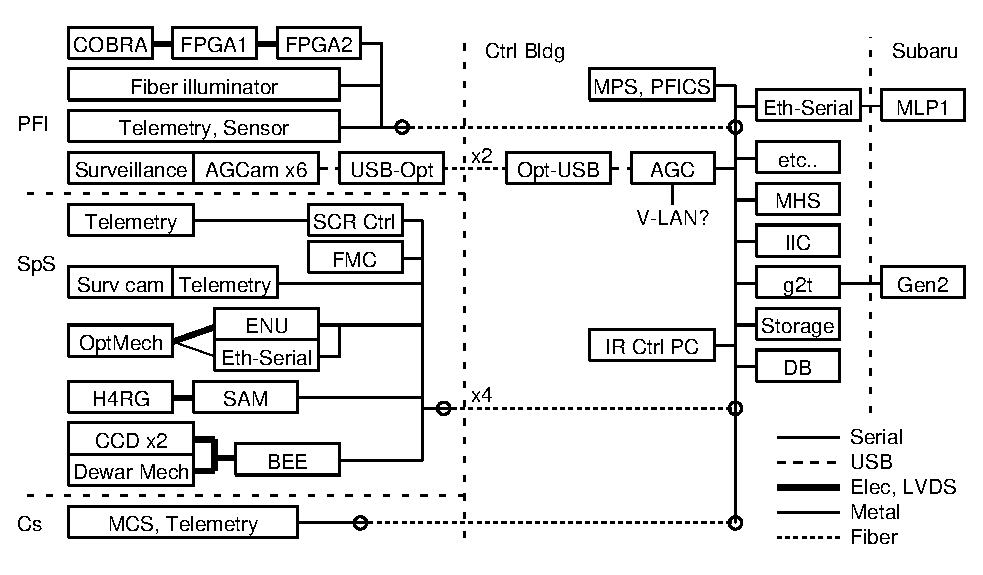
\includegraphics{networks-list.eps}
  \end{center}
  \caption{Schematic network diagram for entire PFS ICS}
  \label{fig:network}
\end{figure}

\subsection{PFI}

\subsubsection{USB over optical fiber / AG cameras}

Current plan is to use 2 pair of dedicated fiber cables for USB over optical 
fiber converter. 
One converter can pass up to four USB connections, and we will use two 
converters for six AG cameras. 
Remaining two USB connections are planned to be used for viewing camera 
and audio input. 

\subsubsection{PFICS/MPS to positioner control}

Current plan is to use UDP between MPS at control building and on-board FPGA 
(FPGA2 in Figure.~\ref{fig:network}). 
Assumed data flow rate is not so high, but RTT to communicate is a key 
to control COBRA positioners. On this point, we are better to 
monitor and control using QoS, and are planning to use PFS-LAN but not E-LAN 
exists at Subaru. 

\subsubsection{Status monitoring and other control commands}

For status monitoring, including environment sensors and monitor hardwares, 
we need to have data connection from some control system to the control 
building. 

Monitoring (viewing) camera and microphone via USB audio will be 
connected via USB-Optical converter, and other sensors and controllers will be 
connedted to ethernet by AVR, PIC etc. 

\subsubsection{Summary}

At least we need to have two pairs of fiber connections which are not 
connected to ethernet, and one ethernet connection. 
For ethernet connection, PFS would like to have dedicated one pair of MM fiber 
connection available for PFS private network. 

Ethernet switch within PFI will be supplied by PFI team (assuming ASIAA)
\footnote{This is due to very limited space and power budget possible for 
control electronics and their cablse within PFI, and selection of network 
boxes need to be considered simultaneously with other mechanical parts and 
structure.}. 

\subsection{Cs / Metrology camera}

Metrology camera (CMOS sensor) will be controlled with Windows box, 
also we will need telemetry sensors and their controller. 
These control boxes will be connected directly to the ethernet. 
Required data rate is not high, since most largest is transferring acquired 
images to archive but not in real time. 

Ethernet switch at Cs will be supplied by IPMU (+Subaru), an interface to 
each control box is an ethernet port (RJ45). 

\subsection{Spectrograph floor}

Due to assumed large data transfer volume and limited number of available 
fibers from SpS floor to control building (via NsIR patch panel), 
network plan and design from SpS floor to control building need to be 
flexible without mass impact to design of SpS floor. 
Therefore we designed SpS floor network in two separated stages: core switch 
to receive connection(s) from control building and to provide connection 
for SpS devices, internal metal ethernet of SpS devices. 

\subsubsection{Spectrograph module within SCR}

\paragraph{Camera control (PU/JHU)}

Each camera unit (xCU\footnote{BCU for blue, RCU for red, NCU for NIR}) 
will output its acquired image and will control 
mechanics and thermal system within each camera (dewar): 

\begin{itemize}
  \item (BCU, RCU) CCD control and readout (BEE)
  \item (NCU) SAM (Sidecar Acquisition Module) for Teledyne H4RG control and readout
  \item Detector focus mechanism (three motors for each xCU)
  \item Cryocooler system (cryotel control, antivibe; 1 for BCU/RCU, 2 for NCU)
  \item Camera thermal control sensor
  \item Vacuum monitoring
\end{itemize}

Latter four systems will be connected by serial or ethernet as shown in 
Figure.~\ref{fig:sps-xcu-control}
\footnote{Note: Active thermal controller seems missing?}, 
external interface is three metal ethernet cables. 

BEE for CCD control and readout is CPU board + FPGA, and connects to 
ethernet and MHS \footnote{An actor will run on this CPU board.} directly. 
No other control box will be required for BCU and RCU at SpS floor nor 
control building. 
SAM for IR detector connects to ethernet, but we will need control PC 
to run tron actor. Since data flow rate for IR up-the-ramp readout will be 
around 300$\sim$500Mbps, we transfer data to the control building directly 
from SAM and have control actor and storage at the control building. 


\begin{figure}[htb]
  \begin{center}
    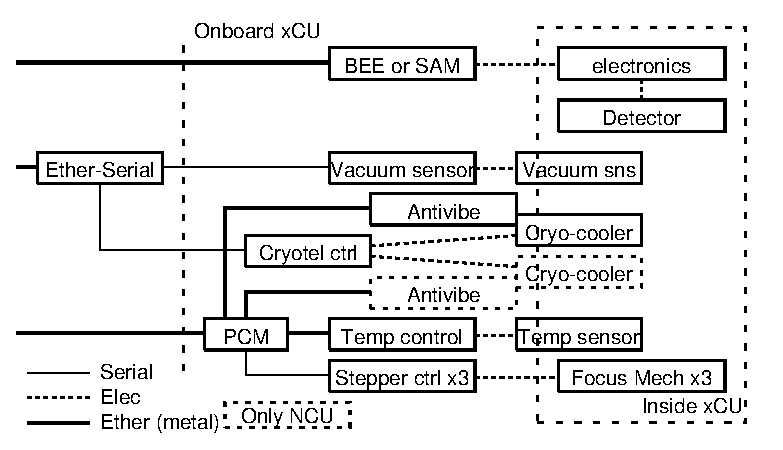
\includegraphics{networks-xcu.eps}
  \end{center}
  \caption{Schematic connection diagram for SpS/SM/xCU
     (Note, detector readout electronics within camera are simplified.)}
  \label{fig:sps-xcu-control}
\end{figure}


\paragraph{Spectrograph module opt-mechanics control (LAM)}

Each spectrograph module has several movable opt-mechanics: 

\begin{itemize}
  \item Dithering mechanism
  \item Slit focusing mechanism
  \item Shutters (Blue, Red)
  \item Back illumination source
  \item Internal illumination source
  \item Red grating exchange mechanism
  \item Enviorment sensors (thermal, pressure, humidity etc.)
\end{itemize}

Slit focusing mechanism is a multi-axis hexapod like stage, and its 
controller requires heavy power load. Only this controller will be mounted 
outside-SCR to reduce heat disipation (power load within SCR). 
All other controllers are connected via serial (RS-232-C), and one ethernet 
to serial converter and control board computer (TBD) 
will be mounted to each SM. 

\paragraph{Telemetery (IPMU)}

Though sensors within thermal enclosure of SM will be provided by LAM, 
this telemetry sensors will monitor other places and will be used for SCR 
temperature control. 

\paragraph{Summary for single SM}

Network design and interface within each single SM is not fixed yet, but 
at least we will have two connections to SpS floor core switch: 
from direct connection from IR-SAM and from others via access switch in 
each SM. 

%To make interface among modules (or institutions), interface within SM have 
%agreed as an port of network switch. 
%At each SM, we will have one ethernet network switch
%\footnote{As (informal) request from Subaru, this switch will be managed.} 
%and two ethernet metal cables will be supplied from SpS core switch, 
%one is for ethernet switch, another directly connects to IR SAM. 
%
%To the ethernet switch at each SM, we will have 11 connections as: 
%\begin{itemize}
%  \item (1) Upstream, to SpS core switch
%  \item (2) CCD-BEE, to BCU and RCU
%  \item (3) xCU ether-serial converter
%  \item (1) Ether-serial converter for SpS opt-mechanics controller
%  \item (3) xCU PCM
%  \item (1) Telemetry (TBD; by IPMU)
%\end{itemize}

\subsubsection{SCR thermal control}

SCR thermal control in detail is not developed yet, current assumptions are: 
\begin{itemize}
  \item to have a controller PC at outside-SCR (rack mount)
  \item to have temperature and humidity sensors over ethernet
    (including telemetries from each SM) 
\end{itemize}


\subsubsection{Control hardware outside SCR}

Total network data rate is dominated by IR up-the-ramp readout which 
is assumed to be $\sim$2Gbps for all four IR detectors, and other data flows 
including CCD readout are not high. 
Including mergin and possibility to separate network subnet, having four 1Gbps 
connections
\footnote{Several implementation plans are under discussion, but baseline is 
to keep at least 4Gbps in total. } 
would be safer. 

Also as infrastructure items at SpS floor, following items are assumed, 
all will be connected via ethernet: 

\begin{itemize}
  \item Core switch (connecting to control building via 4x SM 1Gbps)
  \item Fiber monitoring camera (by LNA)
  \item AC-DC power converter and monitor to supply camera controllers
    (by PU/JHU)
  \item Surveillance camera (TBD: two in SCR, one outside SCR)
  \item PDU
\end{itemize}


\subsubsection{Summary}

We need 4Gbps bandwidth between SpS floor and control building, and 
propose to have four pairs of SM fibers as non-WDM for this
\footnote{Since fiber cables through the telescope structure were made 
at 1990's, these would be G.652 typed SM but not NS-DSF (need to be checked 
with initial specifications), using single core bidirectional mode will 
make risk on operation.}. 
Entire network at SpS floor will be under PFS private network. 

Interfaces among institutions are defined as network port (at switch), 
but not yet defined clearly. 
%and network switches (core and four switches at each SM) will be provided 
%by IPMU (+Subaru). 

\section{Items requested to Subaru}

Following items had requested to Subaru. 
All fibers are from control buidling patch panel. 

\begin{itemize}
  \item (Permitted) To have PFS dedicated ethernet network subnet (PFS-LAN)
  \item (Assigned) 2 pairs of MM fibers to PFI
    (will be used for USB-Optical converter)
  \item (Assigned) 1 pairs of MM fibers to PFI
    (will be used for GbE)
  \item (Assigned\footnote{pfspo:12618}) 
    4 SM fibers (4 pairs or 4 fibers w/WDM) to SpS floor (via NsIR)
  \item 1 SM fibers (1 pairs or 1 fiber w/WDM) to Cs
    \footnote{if SM is not avail, MM is ok}
  \item (Assigned\footnote{pfspo:12618}) 
    1 set of MM fibers to TUE (via NsOpt), same as a set to PFI
\end{itemize}

And following fibers (Table.~\ref{tab:subaru-fiber}) have assigned by Subaru. 
For fiber cables to POpt2, we shall use ones in the same set as HSC. 

\begin{table}[htb]
\begin{center}
\caption{Assigned fibers by Subaru}
\label{tab:subaru-fiber}
\begin{tabular}{c|c|c|c}
to & fiber & mode & remarks \\
\hline
POpt2 & FB17408B & MM 50um & at OCB21: A41J72-A41J71, A41J70-A41J69 (Spare) \\
POpt2 & FB17409B & MM 50um & at OCB21: A41J76-A41J75, A41J74-A41J73 (Spare) \\
POpt2 & FB17412C & MM 62.5um & at OCB21: A41J84-A41J83, A41J82-A41J81 (Spare) \\
\hline
TUE (NsOpt) & FB15315B & MM 50um & (MPO; No spare) \\
TUE (NsOpt) & FB15318C & MM 62.5um & (MPO; 2 for spare) \\
\hline
SpS (NsIR) & FB15404A & SM & (MPO; No spare) \\
SpS (NsIR) & FB15405A & SM & (MPO; No spare) \\
\hline
Cs & Not yet & -- &  \\
\end{tabular}
\end{center}
\end{table}

\subsection{Test and fiber attenuation measurement results} 

\subsubsection{Fiber attenuation measurement method}

We could not prepare suitable calibration code or tail code since 
target connectors at patch panels were MPO, measurements were performed 
like 3-test code method or 1-test code method. 

We measured both patch cables + target and patch cables only. 
Connectors of target fibers are all MPO, we used MPO - 4x SC patch cable on 
each side. Laser outlets of SM/1310nm (CW) and MM/850nm are SC and directly 
connected to MPO-SCx4 patch cables, 
measurements' inlets could catch center cable guide (narrow stick w/fiber 
at its center) directly.
Measurement of patch cables + target are:
{\bf laser outlet - SC - MPO - (target) - MPO - SC - dBm measurement} 
and used MPO-MPO adopter for patch cables' measurement.
We did two measurements per each fiber connection, and rejected / re-measured 
when two have difference more than 1dBm. 
Fiber connectors of patch cables (MPO-SCx4) were cleaned before measurement, 
but we have not cleaned panel connectors. 

\subsubsection{Results}

Results of measurements are in Table~{tab:subaru-measurement}. 
Results for patch cables are subtracted. 

\begin{table}[htb]
\begin{center}
\caption{Measured fiber attenuations (dB)}
\label{tab:subaru-measurement}
\begin{tabular}{c|c|c||r|r|r|r||l}
to & fiber & mode & 1 & 2 & 3 & 4 & remarks \\
\hline
NsOpt & FB15315B & MM/50nm & 1 & 2 & 1 & 1 & Assigned \\
NsOpt & FB15318C & MM/62.5nm & 2 & 1 & 2 & 2 & Assigned \\
NsOpt & FB15319C & MM/62.5nm & 1 & 2 & 2 & 2 & \\
NsOpt & FB15320C & MM/62.5nm & 2 & 1 & 2 & 2 & \\
NsIR & FB15404A & SM & 2.0 & 3.0 & 2.5 & 2.4 & Assigned \\
NsIR & FB15405A & SM & 0.2 & 1.1 & 0.9 & 1.9 & Assigned (Measured by Matt-san) \\
NsIR & FB15406A & SM & 1.6 & 0.9 & 1.9 & 18.4 & \\
NsIR & FB15408A & SM & 1.5 & 0.5 & 2.5 & 1.4 &  \\
NsIR & FB15409A & SM & 1.7 & 1.7 & 3.3 & 1.8 &  \\
NsIR & FB15410A & SM & 0.6 & 1.1 & 1.1 & 0.9 &  \\
\end{tabular}
\end{center}
\end{table}

\end{document}

